The third navigational method we consider was first described by \citet{MenziesAlAkaidi2007a}, and entails computing a new set of ambisonics signals by re-expanding the sound field about a translated expansion center using frequency-domain translation coefficients.

Following the theory described in \secref{sec:02_Acoustical_Theory:Ambisonics_Translation}, the ambisonics signals for the listener, $\mathbf{a}(k)$, are given by
\begin{equation}\label{eq:03_Navigation_Techniques:Forward_Ambisonics_Translation}
\mathbf{a}(k) = \left( \mathbf{T}(k, \vec{r}_0 - \vec{u}) \right)^\text{T} \cdot \mathbf{b}(k),
\end{equation}
where again $\vec{u}$ is the position of the ambisonics microphone (i.e., the expansion center for $\mathbf{b}$) and $\vec{r}_0$ is the position of the listener (cf.~\eqnref{eq:02_Acoustical_Theory:Translated_Expansion_Coefficients_Matrix}).
Recall that the translated expansion coefficients $A_n$ can be computed to an arbitrary order $L_\text{out}$.

The potential field at $\vec{r} + \vec{r}_0$ obtained through translation along $\vec{r}_0 - \vec{u}$ is then given by \eqnref{eq:03_Navigation_Techniques:Output_Potential_Field}.
It is important to note that the re-expanded field is still limited in accuracy and region of validity by the original expansion.
In other words, with increasing $L_\text{out}$, the re-expanded field approaches the original \textit{order-limited} field, not the incident field.

According to the inequality given in \eqnref{eq:01_Introduction:kr_Inequality}, the accuracy of the translated ambisonics signals will degrade with increasing frequency and distance away from the microphone.
To explore this behavior in the frequency domain, we compute the frequency response induced by translation away from the microphone and plot, in \figref{fig:03_Navigation_Techniques:SRE_RollOff}, the magnitude responses corresponding to various translation distances and input orders.%
\footnote{Simulations of this type are described in more detail in \chapref{chap:06_Simulation_Framework}.
Briefly, in this case, the sound field consists of a single point-source placed at $\vec{s}_0 = (2.5, 0, 0)$~m, a microphone of order $L_\text{in} \in [1,5]$ placed at $\vec{u} = (0.25, 0, 0)$~m, and a variable listener position of $\vec{r}_0 = (x_0, 0, 0)$ with $x_0 \in [0, 0.25]$~m.
A diagram of this geometry is shown in \figref{fig:06_Simulation_Framework:Point_Geometry}.
The microphone signals are given by \eqnref{eq:02_Acoustical_Theory:PointSource_An} and we have omitted the near-field compensation high-pass filter defined in \eqnref{eq:02_Acoustical_Theory:NearField_HPF}.
The effective frequency response induced by translating from $\vec{u}$ to $\vec{r}_0$ via \eqnref{eq:03_Navigation_Techniques:Forward_Ambisonics_Translation} is then given by the ratio of the translated zeroth-order ambisonics signal, $A_0(k)$, to the zeroth-order reference ambisonics signal, $B_0(k)$, that would have been measured at $\vec{r}_0$.}
From these plots, we see that translation effectively acts as a low-pass filter, the corner frequency of which approximately corresponds to $k \propto L_\text{in} / \| \vec{r}_0 - \vec{u} \|$.
(Although not shown here, it can be verified that this behavior also holds across all source and listener positions.
See, for example, \figref{fig:07_Characterization_Extrapolation:Azimuth_Dependence:SRE}, which shows this behavior over multiple source azimuths.)

\begin{figure}[t]
  \centering
  \begin{subfigure}[b]{0.49\textwidth}
    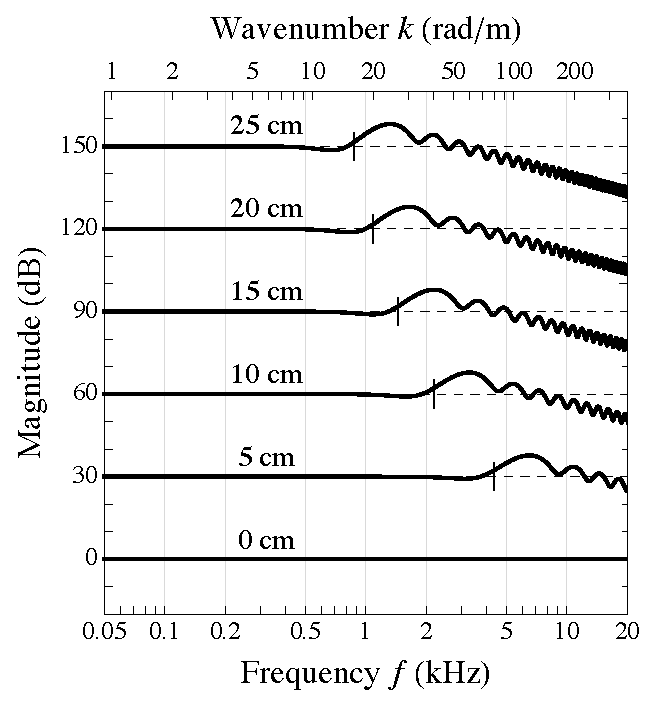
\includegraphics[width=\textwidth]{03_navigational_techniques/figures/freqResp_listenerPos_sre.eps}
    \caption{Varying $\| \vec{r}_0 - \vec{u} \|$; fixed $L_\text{in} = 4$}
    \label{fig:03_Navigation_Techniques:SRE_RollOff:ListenerPos}
  \end{subfigure}
  \hfill
  \begin{subfigure}[b]{0.49\textwidth}
    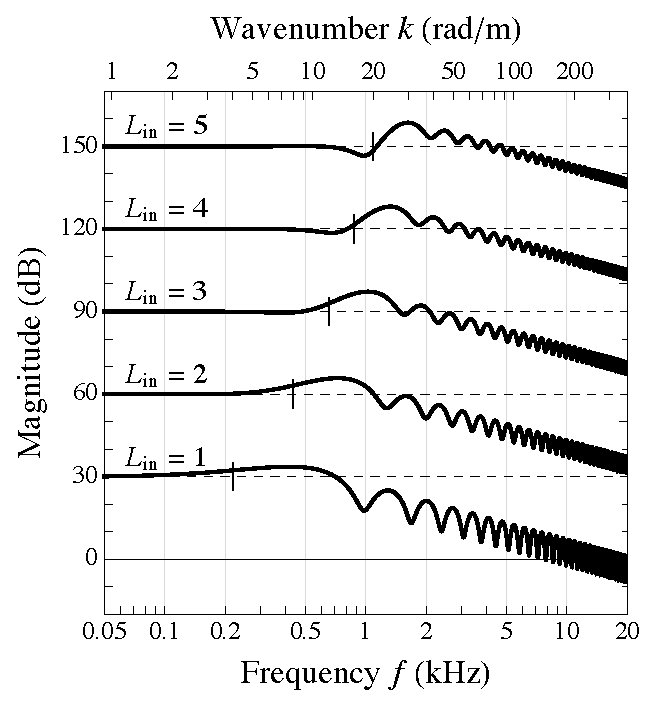
\includegraphics[width=\textwidth]{03_navigational_techniques/figures/freqResp_inputOrders_sre.eps}
    \caption{Varying $L_\text{in}$; fixed $\| \vec{r}_0 - \vec{u} \| = 0.25$~m}
    \label{fig:03_Navigation_Techniques:SRE_RollOff:InputOrders}
  \end{subfigure}
  \caption[Magnitude responses caused by the ambisonics translation method.]{
  Magnitude responses caused by the ambisonics translation method for various translation distances (left panel) and input orders (right).
  The bottom axes show frequency in kHz while the top axes show the angular wavenumber $k$.
  The short vertical lines indicate the nondimensional frequency $k \| \vec{r}_0 - \vec{u} \| = L_\text{in}$.
  For legibility, each frequency response is offset by $30$~dB.}
  \label{fig:03_Navigation_Techniques:SRE_RollOff}
\end{figure} %%NOTE%% vertical axis label is too complicated: |A0 / B0ref| or something

To better show the similarities across these different parameters, we plot, in \figref{fig:03_Navigation_Techniques:Nondim_SRE_RollOff}, the same magnitude responses as in \figref{fig:03_Navigation_Techniques:SRE_RollOff}, but now against a normalized wavenumber, $k \| \vec{r}_0 - \vec{u} \| / L_\text{in}$.
As expected, the corner of each effective low-pass filter is located at $k \| \vec{r}_0 - \vec{u} \| / L_\text{in} \approx 1$.
From these plots, we clearly see that the basic shape of the magnitude response is virtually identical across different translation distances (see \figref{fig:03_Navigation_Techniques:Nondim_SRE_RollOff:ListenerPos}), whereas varying the input order yields noticeable differences (\figref{fig:03_Navigation_Techniques:Nondim_SRE_RollOff:InputOrders}).
In particular, increasing the input order decreases the amplitude of, and spacing between, the ``ripples'' that modulate the overall low-pass behavior above the corner.

\begin{figure}[t]
  \centering
  \begin{subfigure}[b]{0.49\textwidth}
    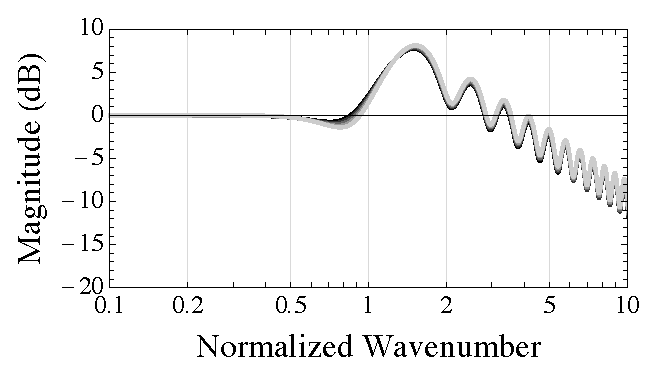
\includegraphics[width=\textwidth]{03_navigational_techniques/figures/nondimFreqResp_listenerPos_sre.eps}
    \caption{Varying $\| \vec{r}_0 - \vec{u} \|$; fixed $L_\text{in} = 4$}
    \label{fig:03_Navigation_Techniques:Nondim_SRE_RollOff:ListenerPos}
  \end{subfigure}
  \hfill
  \begin{subfigure}[b]{0.49\textwidth}
    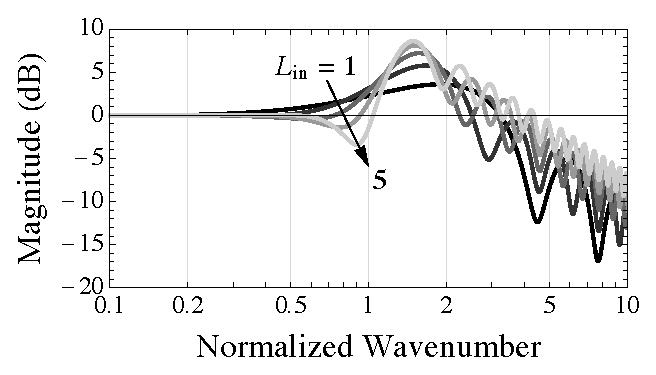
\includegraphics[width=\textwidth]{03_navigational_techniques/figures/nondimFreqResp_inputOrders_sre.eps}
    \caption{Varying $L_\text{in}$; fixed $\| \vec{r}_0 - \vec{u} \| = 0.25$~m}
    \label{fig:03_Navigation_Techniques:Nondim_SRE_RollOff:InputOrders}
  \end{subfigure}
  \caption[Magnitude responses caused by the ambisonics translation method.]{
  Magnitude responses caused by the ambisonics translation method for various translation distances (left panel) and input orders (right), where the lighter gray curves correspond to increasing translation distance or input order, respectively.
  The horizontal axes show the nondimensional wavenumber $k \| \vec{r}_0 - \vec{u} \| / L_\text{in}$.}
  \label{fig:03_Navigation_Techniques:Nondim_SRE_RollOff}
\end{figure}

It is worth noting that translation may also be carried out through the \textit{inverse} (or pseudoinverse if $L_\text{in} \neq L_\text{out}$) operation, such that
\begin{equation}\label{eq:03_Navigation_Techniques:Inverse_Ambisonics_Translation}
\mathbf{a}(k) = \left(\left( \mathbf{T}(k, \vec{u} - \vec{r}_0) \right)^\text{T} \right)^{-1} \cdot \mathbf{b}(k).
\end{equation}
However, as shown in \figref{fig:03_Navigation_Techniques:SRE_RollOff}, the forward translation operation given by~\eqnref{eq:03_Navigation_Techniques:Forward_Ambisonics_Translation} leads to an attenuation (i.e., a ``roll-off'') of high frequencies.
Consequently, the inverse operation will yield excessive high-frequency amplification, unless steps (such as regularization) are taken to mitigate such excessive gains.

In \secref{sec:03_Navigation_Techniques:Pinv_Technique}, a regularized least-squares approach is implemented in an interpolation method that uses multiple ambisonics microphones to estimate the ambisonics signals at the position of the listener.
Consequently, the inverse approach to extrapolation defined in \eqnref{eq:03_Navigation_Techniques:Inverse_Ambisonics_Translation} can be considered a special case of that interpolation method, in which we have only a single array (i.e., $P = 1$) and no regularization is used.